Para la función, $f(x)$, cuya gráfica está dada, determine, si existe, cada límite indicado. En caso que no exista, justifique su respuesta.

\begin{figure}[H]
    \centering
    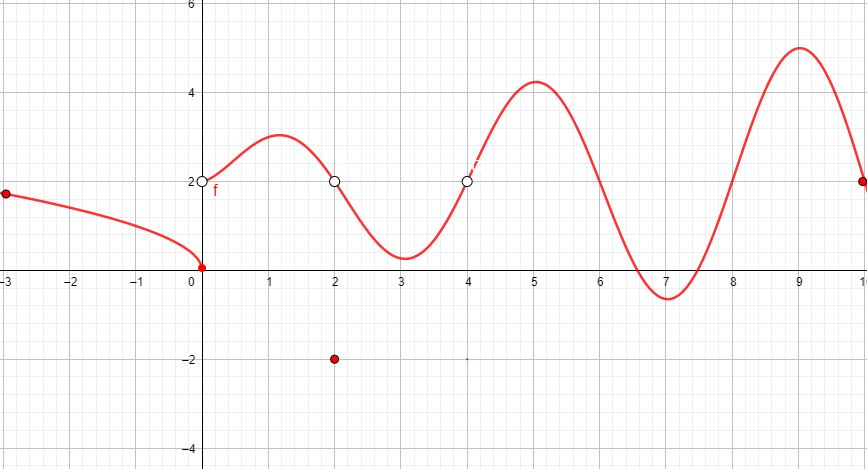
\includegraphics[scale=0.65]{problema_1.png}
    \label{fig:problema_1}
\end{figure}

\begin{soluciones}
    \subsubsection*{Solución}

    \begin{enumerate}[label=\alph*)]
        \item $\ds\lim_{x \rightarrow 2} f(x)=2$
        \item $\ds\lim_{x \rightarrow 4} f(x)=2$
        \item $\ds\lim_{x \rightarrow 0} f(x)=$ no existe ya que $\ds\lim_{x \rightarrow 0^{-}} f(x)=0 \neq \ds\lim_{x \rightarrow 0^{+}} f(x)=2$
    \end{enumerate}
\end{soluciones}